%%%% Better Poster latex template example v1.0 (2019/04/04)
%%%% GNU General Public License v3.0
%%%% Rafael Bailo
%%%% https://github.com/rafaelbailo/betterposter-latex-template
%%%%
%%%% Original design from Mike Morrison
%%%% https://twitter.com/mikemorrison

\documentclass[alleghenyposter]{betterposter}

\usepackage{comment}
\usepackage{amsmath}
\usepackage{amssymb}
\usepackage{url}
\usepackage{graphicx}

% custom packages
\usepackage{fancyhdr}
\usepackage{hyperref}
\usepackage{subcaption}
\usepackage{mathtools}
\usepackage{mathptmx}
\usepackage{listings}
\usepackage{mdframed}
\usepackage{tikz}

%%%% Uncomment the following commands to customise the format

%% Setting the width of columns
% Left column
%\setlength{\leftbarwidth}{0.25\paperwidth}
% Right column
%\setlength{\rightbarwidth}{0.25\paperwidth}

%% Setting the column margins
% Horizontal margin
%\setlength{\columnmarginvertical}{0.05\paperheight}
% Vertical margin
%\setlength{\columnmarginhorizontal}{0.05\paperheight}
% Horizontal margin for the main column
%\setlength{\maincolumnmarginvertical}{0.15\paperheight}
% Vertical margin for the main column
%\setlength{\maincolumnmarginhorizontal}{0.15\paperheight}

%% Changing font sizes
% Text font
%\renewcommand{\fontsizestandard}{\fontsize{28}{35} \selectfont}
% Main column font
%\renewcommand{\fontsizemain}{\fontsize{28}{35} \selectfont}
% Title font
%\renewcommand{\fontsizetitle}{\fontsize{28}{35} \selectfont}
% Author font
%\renewcommand{\fontsizeauthor}{\fontsize{28}{35} \selectfont}
% Section font
%\renewcommand{\fontsizesection}{\fontsize{28}{35} \selectfont}

%% Changing font sizes for a specific text segment
% Place the text inside brackets:
% {\fontsize{28}{35} \selectfont Your text goes here}

%% Changing colors

\definecolor{boldgold}{RGB}{254,218,72} % Bold Gold
\definecolor{teal}{RGB}{0,117,122} % Teal
\definecolor{glassgreen}{RGB}{0,169,183} % Glass Green
\definecolor{brightblue}{RGB}{0,123,195} % Bright Blue
\definecolor{acblue}{RGB}{0,33,68} % AC Blue


% Background of side columns
\renewcommand{\columnbackgroundcolor}{white}
% Font of side columns
\renewcommand{\columnfontcolor}{black}
% Background of main column
\renewcommand{\maincolumnbackgroundcolor}{acblue}
% Font of main column
\renewcommand{\maincolumnfontcolor}{white}

\begin{document}
\betterposter{
%%%%%%%% MAIN COLUMN

\maincolumn{
%%%% Main space
\vspace{-3in}
\textbf{RayTerm} is a \textbf{tool} to aid the creation of \textbf{graphical applications} in a \textbf{Terminal}

\vspace{3in}
\begin{center}
  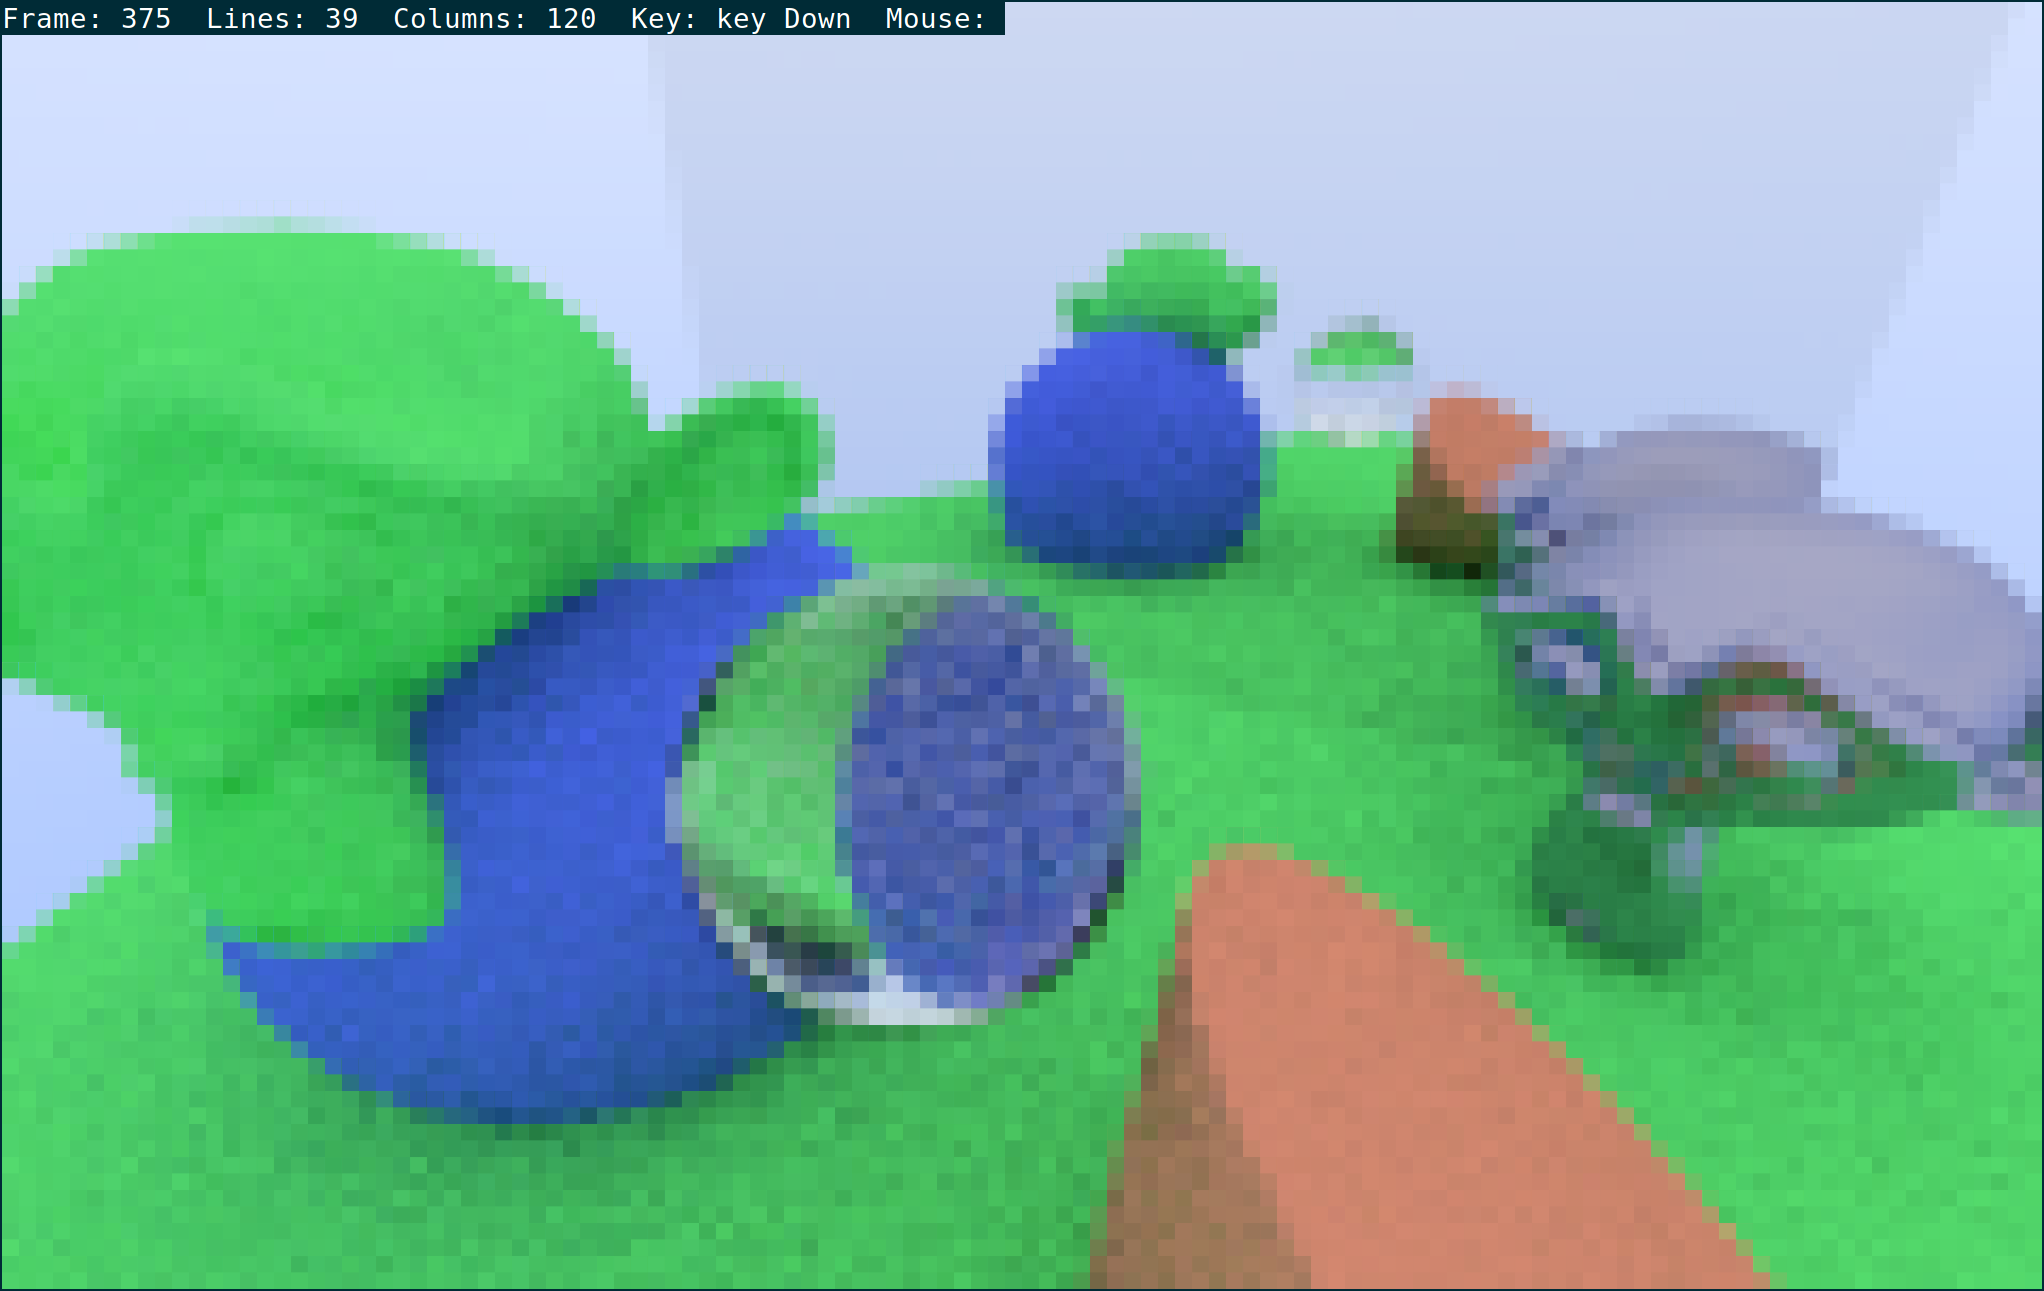
\includegraphics[width=0.98\textwidth]{img/rayterm}
\end{center}
\vspace{-3in}
}{
%%%% Bottom-left space

\qrcode{img/qrcode}{img/smartphoneWhite}{
\textbf{Scan the QR code} to
\\download the full paper
}

}{
%%%% Bottom-right space


\begin{minipage}[c]{0.5\textwidth}
\begin{center}
{ \fontsize{16}{22} \selectfont Rendered 7 objects in 455 seconds on a CPU }
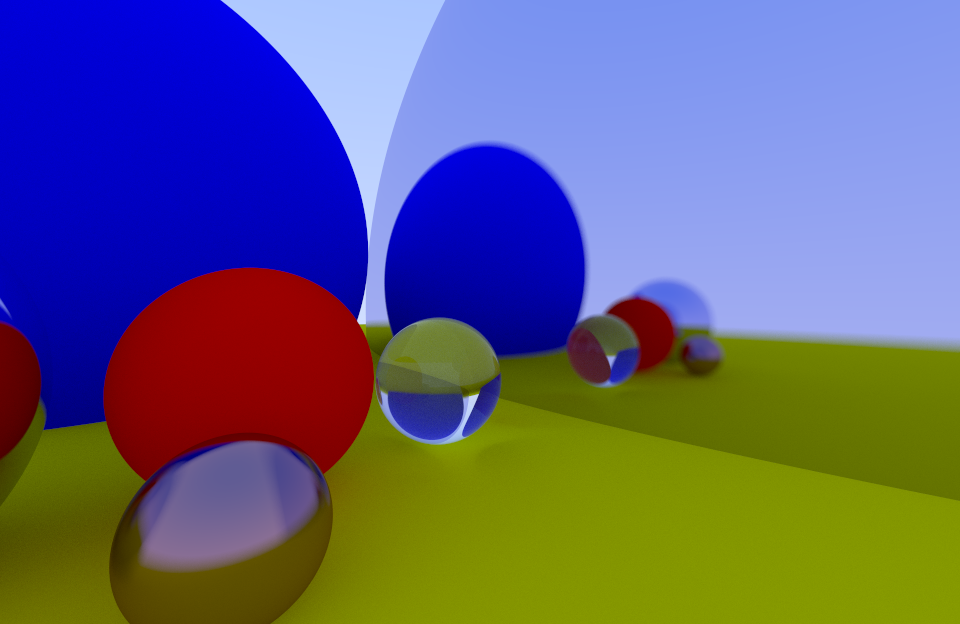
\includegraphics[width=0.9\textwidth]{img/hq-cpu}
\end{center}
\end{minipage}%
\begin{minipage}[c]{0.5\textwidth}
\begin{center}
{ \fontsize{16}{22} \selectfont Rendered 46,914 objects in \textasciitilde{}20 seconds on a GPU }
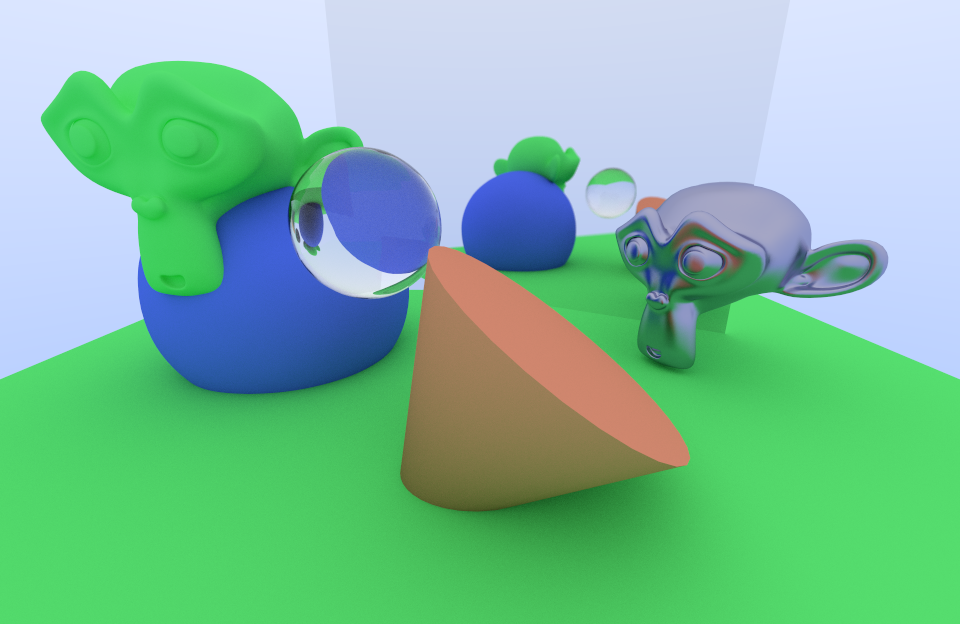
\includegraphics[width=0.9\textwidth]{img/hq-gpu}
\end{center}
\end{minipage}%
}

}{
%%%%%%%% LEFT COLUMN

\title{RayTerm}
\subtitle{A Ray-Tracing Rendering Engine for XTerm-like Terminals}
\author{Saejin Mahlau-Heinert}
\institution{CMPSC \& Studio Art, Allegheny College}
\author{Janyl Jumadinova}
\institution{CMPSC Professor, Allegheny College}
\author{Gregory Kapfhammer}
\institution{CMPSC Chairman, Allegheny College}

\section{What is RayTerm}
RayTerm is a C++ ray-tracing library that is performant, open-source, and programmable.
Its aesthetic is both retro and futuristic: old pixilated graphics are combined with photorealistic lighting.

\section{Purpose}
RayTerm is designed for other programmers --- the library simplifies the development of terminal-based programs.
These terminal programs are often preferred by artists and developers, allowing easy access to many content types.


\section{Challenge}
Real-time rendering is difficult because each frame must be rendered in less than thirty milliseconds; otherwise movement seems choppy and under-sampled.
Ray-tracing is a computationally intensive process, however, and so optimization and parallelization is needed.

%% This fills the space between the content and the logo
\vfill


\includegraphics[width=\textwidth]{img/allegheny-logo}\\

}{
%%%%%%%% RIGHT COLUMN

\section{Ray-Tracing}
Ray-tracing is a method to simulate the path that photons take through the world.

\begin{center}
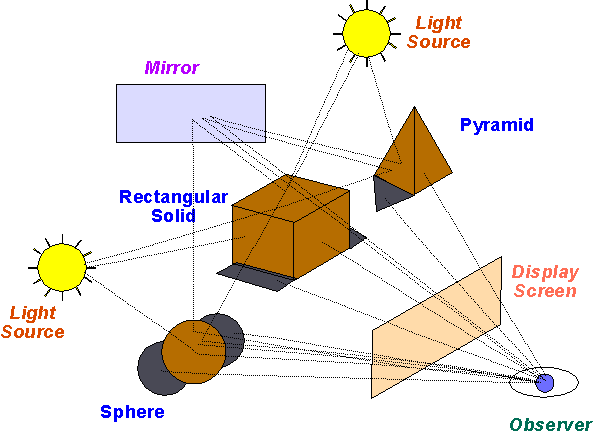
\includegraphics[width=0.75\textwidth]{img/world}
\end{center}

\section{The Rendering Equation}
\vspace{-1.5em}
\begin{center}
$I(x, x') = g(x, x') \Big[\epsilon(x, x') + \int_{S} \rho(x, x',x'')I(x', x'')dx''\Big]$
\end{center}

\section{Materials}
Light bouncing between surfaces gives the world its color and feel.
In RayTerm `materials' model this bouncing.

\begin{center}
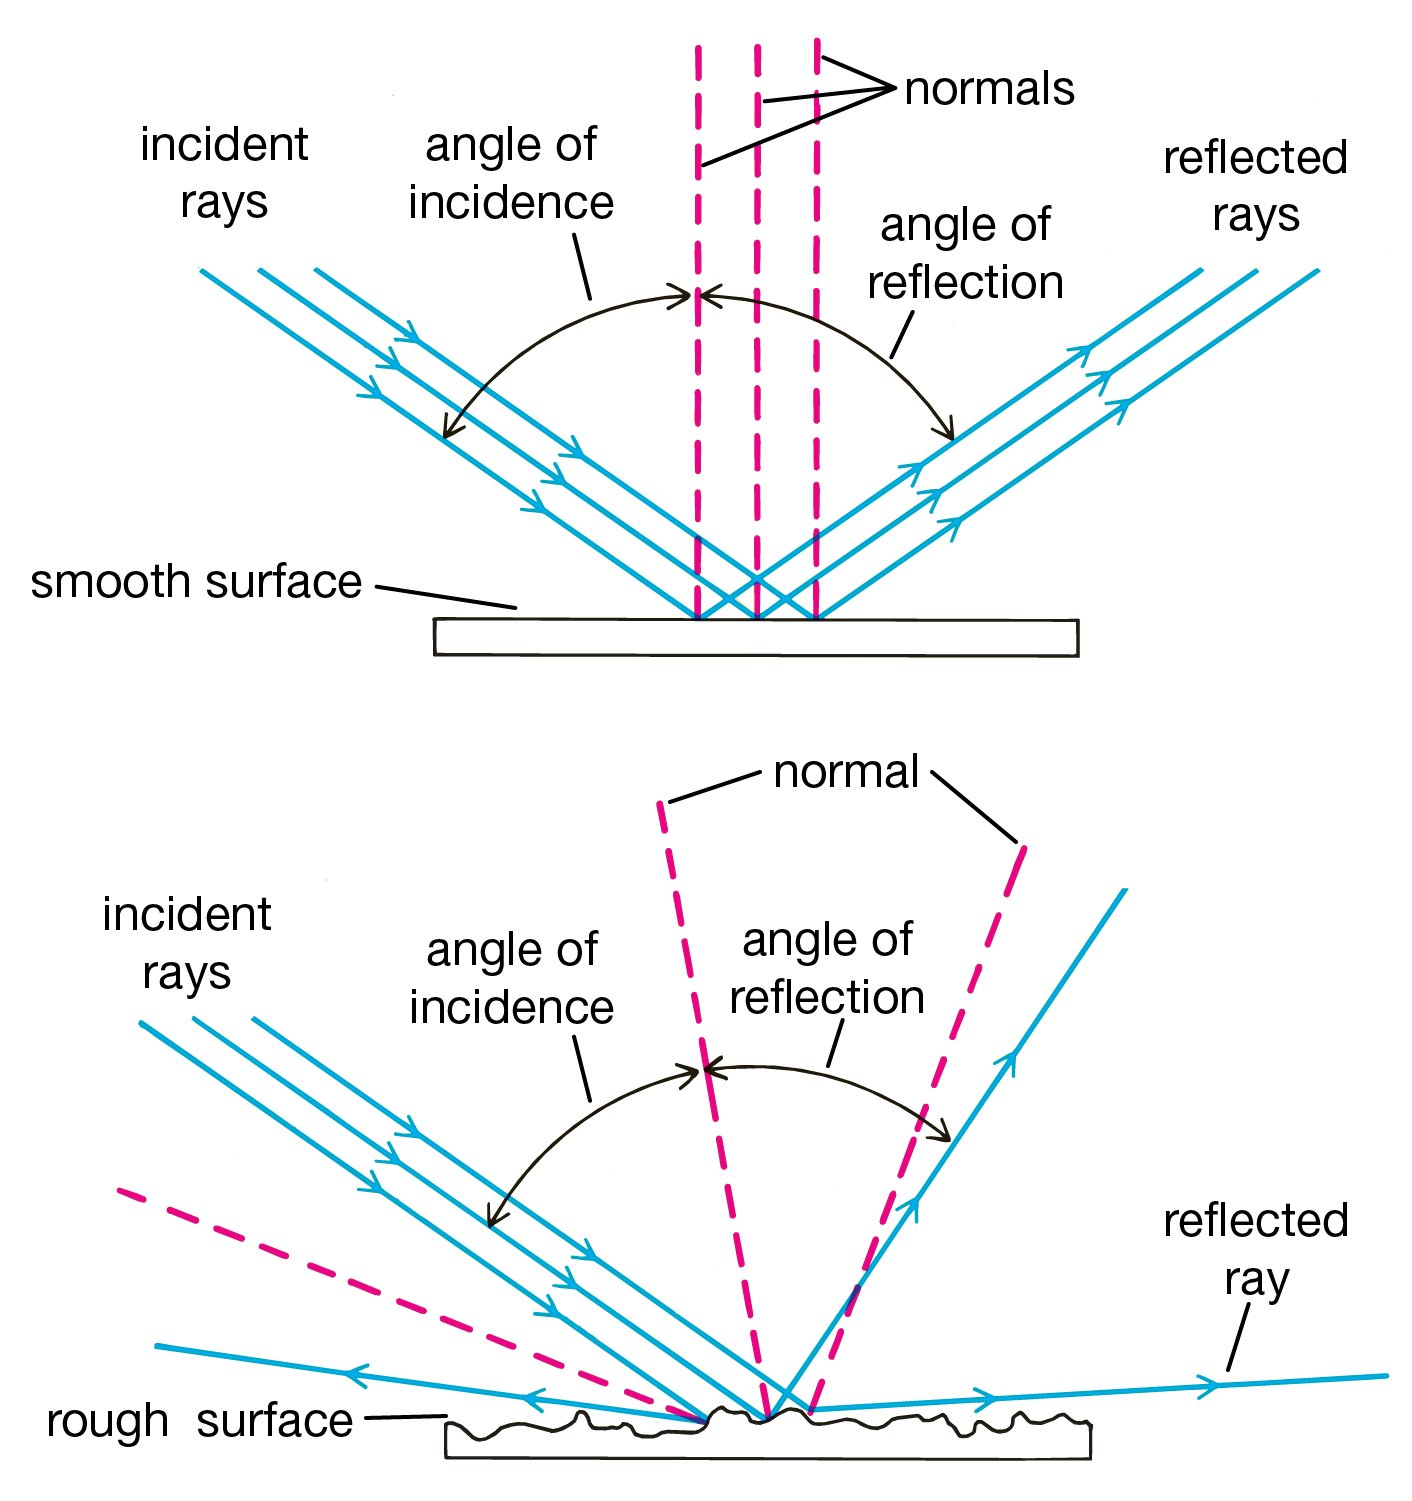
\includegraphics[width=0.75\textwidth]{img/surface}
\end{center}

\section{RTExplore}
The main image to the left was produced by \texttt{rtexplore}, an example application of about 130 lines of code built with RayTerm.
%% This fills the space between the content and the logo
\vfill


\includegraphics[width=\textwidth]{img/cmpsc-logo}\\

}
\end{document}
